\documentclass{article}
\usepackage{algorithm2e}
\usepackage{float}
\usepackage{graphicx}

\title{CME 211 PROJECT REPORT}
\author{Emmanuel Anifowose}
\date{November 18, 2020}

\begin{document}
\setlength{\parindent}{0pt}
\setlength{\parskip}{1ex}

\maketitle

\section{Introduction}
This project develops a program to solve the 2D heat equation on a simple geometry
using a sparse matrix solver written in C++. The method used to solve the equation
numerically is the \emph{finite-difference} method. For the geometry given in the project,
the resulting system of equations is symmetric negative definite hence, the Conjugate
Gradient (CG) method which is an efficient iterative algorithm for this system is
used to solve the equation\cite{CME211:2020:ProjectPart1}.\\
The heat transfer problem to be solved is a system where one is transferring some hot
fluid, with temperature $T_h$, within a pipe. To keep the exterior of the pipe cool,
a series of cold air jets, with temperature $T_c$, are equally distributed along the
pipe and continuously impinge on the pipe surface. The goal is to find the mean
temperature and the temperature distribution within the pipe walls
\cite{CME211:2020:ProjectPart2}.

\section{Description of CG Solver Implementation}
The implementation of CG Solver is carried out using the OOP design approach in C++.
The OOP design uses two classes: \emph{SparseMatrix} and \emph{HeatEquation2D}.\\ The
sparse matrix class defines a sparse matrix object which contains the vectors defining
the matrix as data attributes and methods to perform necessary tasks (add entries,
conversion from COO to CSR format). The HeatEquation2D class contains data and methods
required to form the system of equations, solve the system and output results to files
\cite{CME211:2020:ProjectPart2}.
The pseudocode for the algorithm for the CG Solver can be found below
\cite{CME211:2020:ProjectPart1}.\\

\begin{algorithm}[H]
 \SetAlgoLined
 \KwData{a CSR matrix, a vector, a guess of the solution, tolerance}
 \KwResult{solution of a CSR matrix vector equation}
 initialize $u_0$\;
 $r_0 = b - A$ $u_0$\;
 $L2normr0 = L2norm(r_0)$\;
 $p_0 = r_0$\;
 $niter = 0$\;
 \While{$(niter < nitermax)$}{
  niter = niter + 1\;
  $alpha = (r_n^T$ $r_n)/(p_n^T$ $A$ $p_n)$\;
  $u_{n+1} = u_n + alpha_n$ $p_n$\;
  $r_{n+1} = r_n - alpha_n$ $A$ $p_n$\;
  \If{($L2normr/L2norm0 < threshold)$}{
   break\;
  }
  $beta_n = (r_{n+1}^T$ $r_{n+1})/(r_n^T$ $r_n)$\;
  $p_{n+1} = r_{n+1} + beta_n$ $p_n$\;
 }
 \caption{Conjugate Gradient pseudo-code}
\end{algorithm}
In the implementation of CGSolver, five functions were used to improve readability
of the code.\\
\textbf{L2norm} $-$ This was used to calculate the L2-norm of a vector.\\
\textbf{dotProduct} $-$ This was used to calculate the dot product of two vectors.\\
\textbf{matVecProduct} $-$ This was used to calculate the matrix vector product of a
CSR matrix and a vector.\\
\textbf{scalVecProduct} $-$ This was used to calculate the product of a vector and a
scalar.\\
\textbf{sum2Vec} $-$ This was used to get the sum of two vectors.\\
The use of these functions greatly reduced the length of the code and made
debugging easier.

\section{Users Guide}
\begin{enumerate}
\item A command of \emph{\$ make} to the terminal will compile the code.
\item A command of \emph{\$ ./main [input file] [solution file prefix]} will execute
the code and output solution files for every 10 iterations of CG Solver including the
first and last iterations.
\item A command of \emph{\$ python3 postprocess.py [input file] [solution file]} will
compute the mean temperature in the pipe and create a pseudocolor plot that shows
the temperature distribution in the pipe for that solution file.
\item A command of \emph{\$ python3 bonus.py [input file] [solution file prefix]} will
create an animation of the temperature development during the CG Solve.
\end{enumerate}

\begin{figure}[H]
\centering
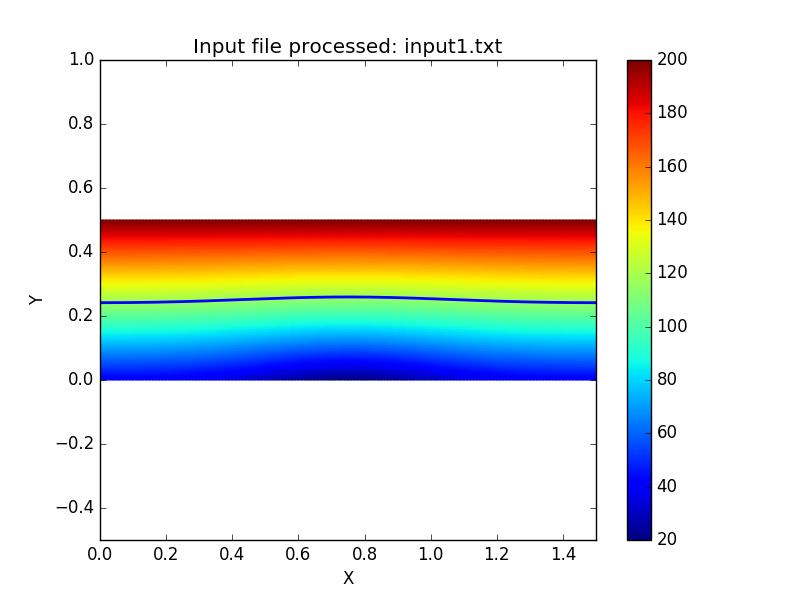
\includegraphics[scale=0.6]{pcolor1.png}
\caption{Example of pseudocolor plot with mean temperature isoline for input1.txt}
\label{fig:pcolor1}
\end{figure}

\bibliographystyle{plain}
\bibliography{references}

\end{document}

//--documentation_-1
//--Well written. Impressive tex/pdf.
//--END
